
\mysubsection{Commande Angulaire et Cartésienne}
Pour la commande dans l'espace des articulations, on a mis en oeuvre sur Matlab et Simulink les deux techniques qu'on a montrés dans les subsections \ref{Comm_Ang} e \ref{Comm_Cart}%\todo{citar seção de metodologia/consigne angular e cartesiana/ consigne angular}
. Ensuite, on a comparé les deux résultats pour choisir la méthode de commande la plus adaptée à notre solution.

Pour les deux simulations, on a choisi la pulsation de brisure $ \omega$ = $ 10$ $rad/s $ %\todo{formula omega = 10 rad/s}
 pour toutes les articulations. Si on augmente la fréquence de brisure, on peut réduire le temps de réponse du système, alors on choisira ce temps d'une façon définitive quand l'intégration avec les autres parties du projet serait fait, pour meilleur adapter la commande au robot. Pour des critères de comparaison, on utilisera les mêmes pulsations de brisure pour tous les tests.

Dans la suite, on a les résultats obtenus pour la commande PID, avec une consigne en échelon de %\todo{vector: [0, pi, -pi/2, -pi/2, 0]}
$ \left[0, -\frac{\pi}{2} , 0, 0, 0 \right] $ filtré par un filtre de primier ordre de constant de temps 0.5s, et les efforts de contrôle nécessaires sur chaque articulation.

\begin{figure}[H]
	\begin{center}	
		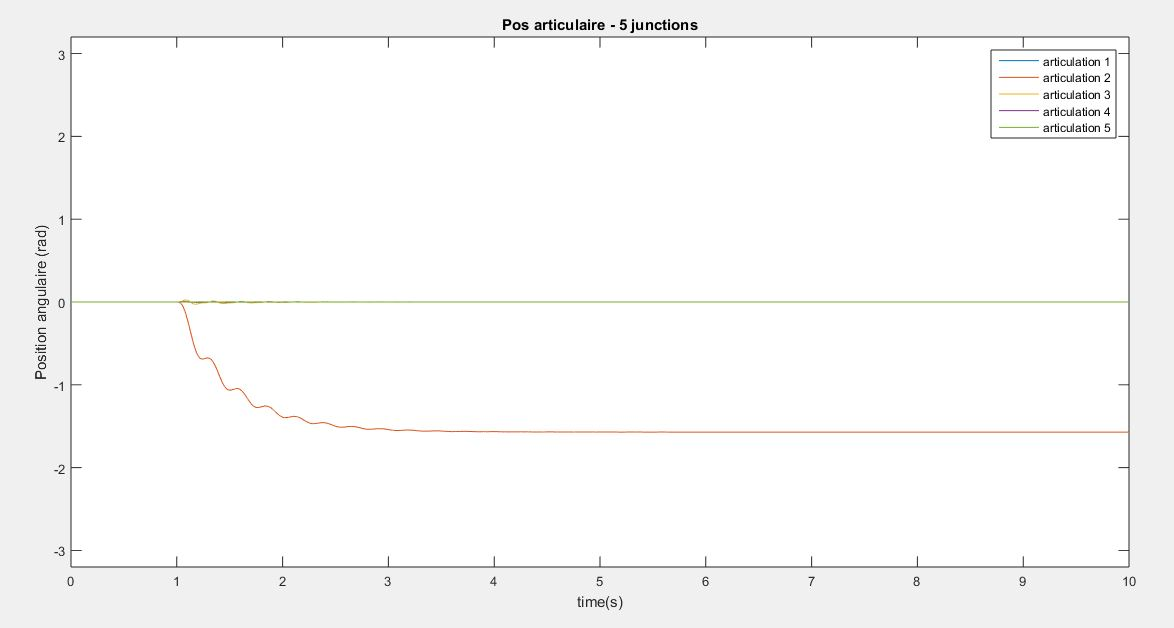
\includegraphics[width=\textwidth]{./PIDjointgraph.JPG}
		\caption{Réponse temporelle à un échelon de consigne pour le système dans l'espace articulaire commandé pour un PID}
		\label{fig:PID_joint_space_response}
	\end{center}
\end{figure}
%\todo{inserir figura: PID joint space response}
%\todo{legenda da figura: Réponse temporelle à un échelon de consigne pour le système dans l'espace articulaire commandé pour un PID}

\begin{figure}[H]
	\begin{center}	
		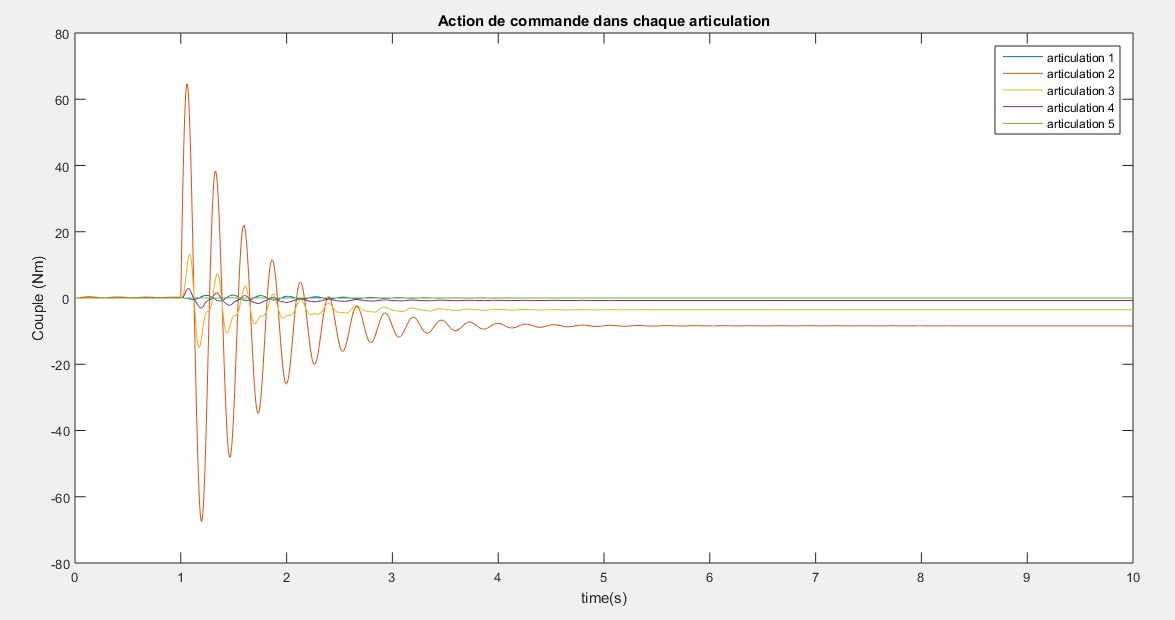
\includegraphics[width=\textwidth]{./PIDjointcontgraph.JPG}
		\caption{Efforts de contrôle pour le système commandé pour un PID dans l'espace articulaire }
		\label{fig:PIDjointcontgraph}
	\end{center}
\end{figure}

On peut noter dans le graphique que le temps de réponse du système est d'environ 2 secondes et l'erreur statique est nulle, ce qui était attendu une fois qu'on a un contrôleur avec un terme intégrale. Cependant, la réponse contienne beaucoup de fluctuations, on croit en raison des non-linérité du système. Pour le efforts de contrôle, il y a aussi beaucoup de fluctuation et ils sont trop grandes dans le début du mouvement.  Alors, cette méthode de commande a quelques problèmes qu'on doit corriger si on l'utilise dans le robot.

Pour la commande PID avec compensation des non-linérités, on a utilisé la même consigne que dans le cas précédent. Dans la suite, on a le graphique qu'on a obtenu dans la simulation pour les position angulaires et les efforts de contrôle.

\begin{figure}[H]
	\begin{center}	
		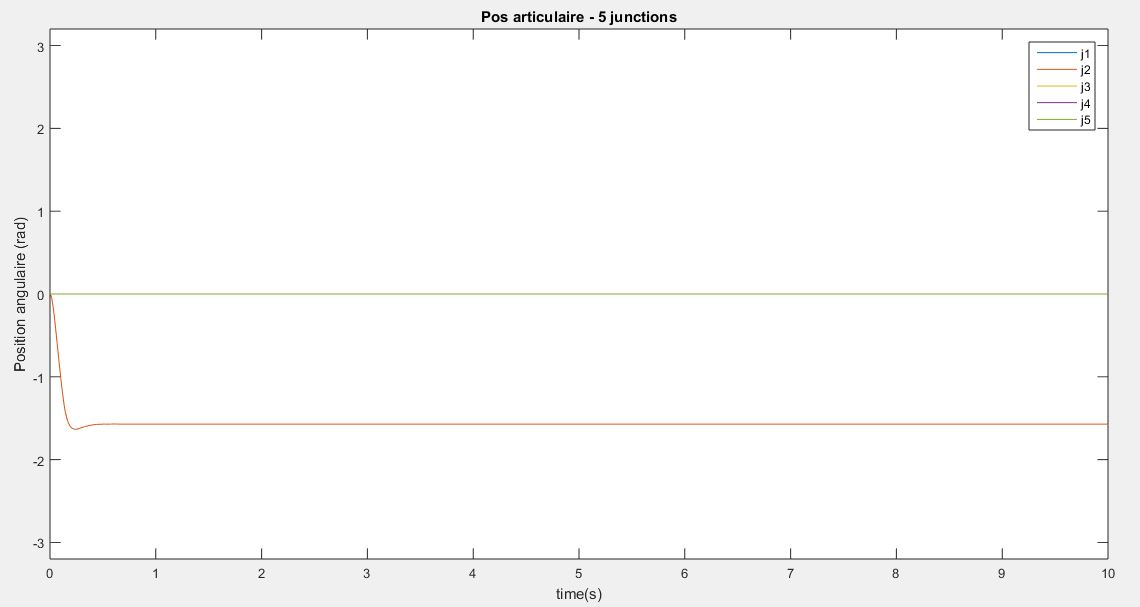
\includegraphics[width=\textwidth]{./CTI_joint_space_response.JPG}
		\caption{Réponse temporelle à un échelon de consigne pour le système dans l'espace articulaire commandé pour un PID avec compensation des non-linéarités.}
		\label{fig:CTI_joint_space_response}
	\end{center}
\end{figure}
%\todo{inserir figura: CTI joint space response}
%\todo{legenda da figura: Réponse temporelle à un échelon de consigne pour le système dans l'espace articulaire commandé pour un PID avec compensation des non-linéarités et sans action intégrale pour des erreurs faibles.}

\begin{figure}[H]
	\begin{center}	
		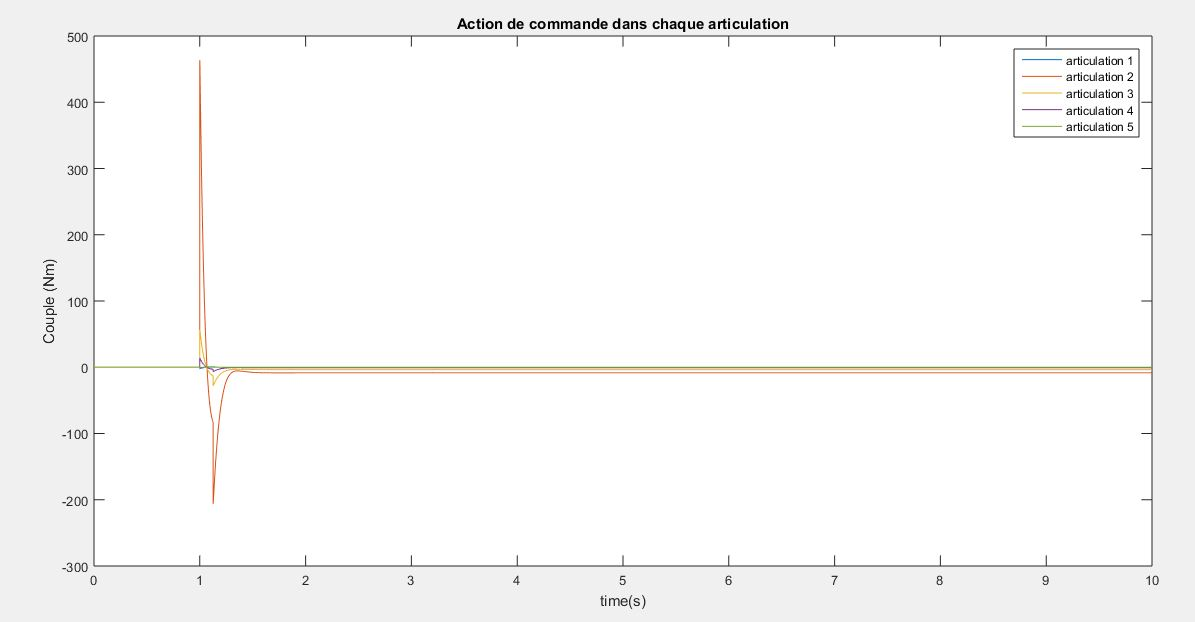
\includegraphics[width=\textwidth]{./CTIgraphcont.JPG}
		\caption{Efforts de contrôle pour le système commandé pour un PID avec compensation des non-linéarités dans l'espace articulaire.}
		\label{fig:CTIgraphcont}
	\end{center}
\end{figure}

On peut noter, comme dans le cas du contrôleur PID, que l'erreur statique est nulle en raison du terme intégrale et le temps de réponse est aussi environ 2 secondes. Cependant, on a réduit considérablement les fluctuations, une fois que les non-linéarités du système sont compensées dans le contrôleur. Par contre, on peut voir que les eeforts de contrôle sont beaucoup plus abrupt au début pour assurer ce comportement au système.

On peut voir aussi que ces réponses semple trop bien parce qu'il s'agit des réponses à une modèle simulé du robot. Dans un cas réel, on n'aura pas accès à la vitesse angulaire et on aura aussi des bruits de mesure et des  incertitudes du modèle estimé. Alors, on a simulé à nouveau ce modèle en ajoutant un bruit blanche à la mesure de position et en déterminant de façon numérique la vitesse angulaire du robot. Les résultats sont dans la suite.

\begin{figure}[H]
	\begin{center}	
		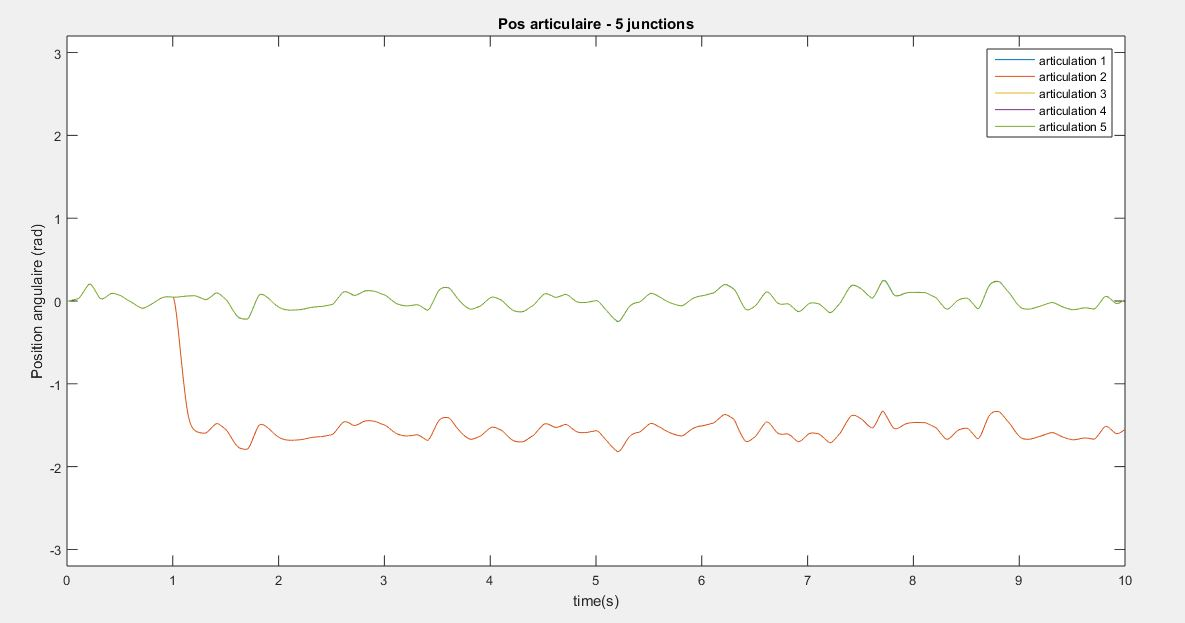
\includegraphics[width=\textwidth]{./CTIdistpos.JPG}
		\caption{Réponse temporelle à un échelon de consigne pour le système dans l'espace articulaire commandé pour un PID avec compensation des non-linéarités et en simulant des bruits de mesure.}
		\label{fig:CTIdistpos}
	\end{center}
\end{figure}
%\todo{inserir figura: CTI joint space response}
%\todo{legenda da figura: Réponse temporelle à un échelon de consigne pour le système dans l'espace articulaire commandé pour un PID avec compensation des non-linéarités et sans action intégrale pour des erreurs faibles.}

\begin{figure}[H]
	\begin{center}	
		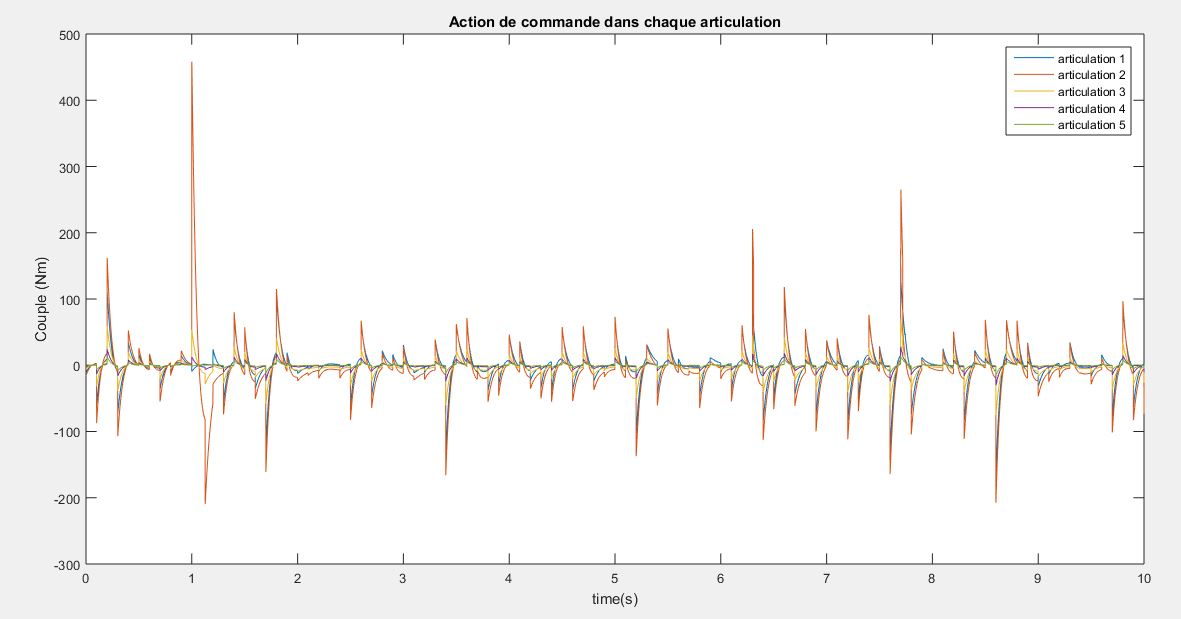
\includegraphics[width=\textwidth]{./CTIdistcont.JPG}
		\caption{Efforts de contrôle pour le système commandé pour un PID avec compensation des non-linéarités dans l'espace articulaire et en simulant des bruits de mesure.}
		\label{fig:CTIdistcont}
	\end{center}
\end{figure}

On peut voir que, pour la position angulaire, cette méthode semble bien même avec des bruits, mais pour l'efforts de contrôle, il y a plusieurs pics de couple trop grande. Alors, cela peut endommager le robot. On conclut que il n'es pas une bonne idée d'utiliser les consignes de vitesse, parce que les bruits de mesures génèrent des pics abruts quand on fait l'estimation numérique.

Pour la commande dans l'espace opérationnel, on a aussi essayé de mettre en oeuvre les deux techniques de commande, mais on s'est rendu compte que l'approche du couple calculé ne marcherait pas bien. On a besoinde calculer da dérivé et la pseudo-inverse du Jacobien pour cette approche, alors si le robot a des variations abrupts de position, le dérivé du Jacobien sera trop grande. Le même pour la pseudo-inverse si le robot est proche d'un point de singularité. Alors, à la fin, on a mis en oeuvre juste l'approche du PID.

On a essayé comme consigne de position $ \left[X,Y,Z\right] $ = $ \left[0.2, 0.2, -0.1\right] $, aussi un échellon filtré par un filtre de premier ordre. Les réponses angulaire et cartésien et les efforts de contrôle sont montrés dans les figures suivantes.


\begin{figure}[H]
	\begin{center}	
		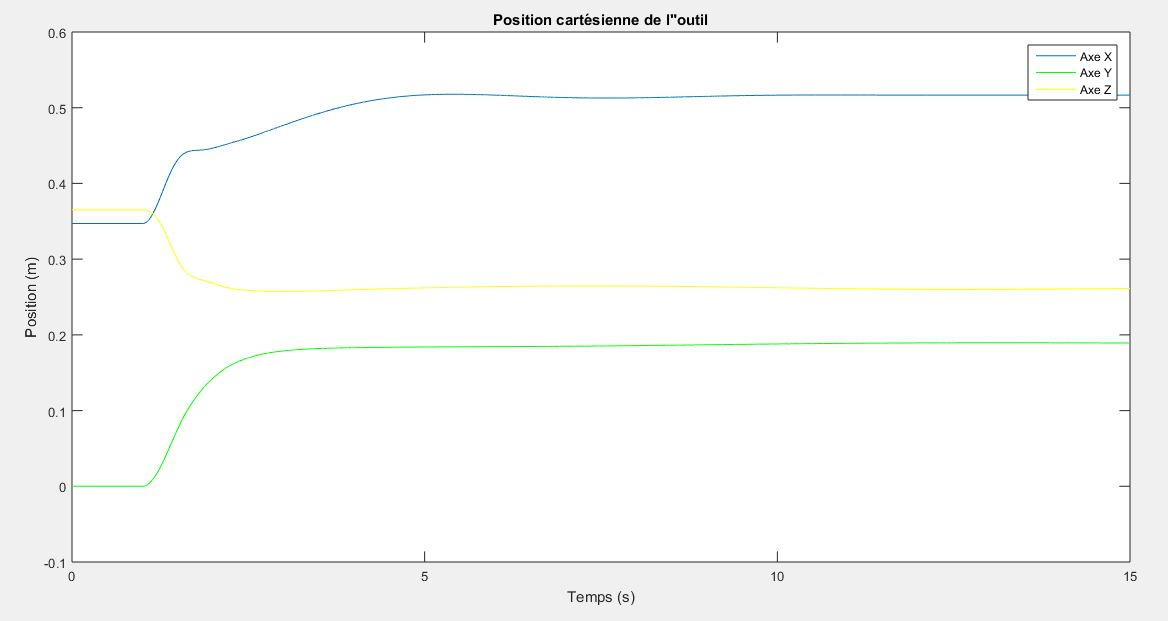
\includegraphics[width=\textwidth]{./PIDtaskxyzgraph.JPG}
		\caption{Réponse temporelle des positions du robot à un échelon filtré de consigne pour le système dans l'espace opérationnel.}
		\label{fig:PIDtaskxyzgraph}
	\end{center}
\end{figure}
%\todo{inserir figura: Operational space response}
%\todo{legenda da figura: Réponse temporelle à un échelon de consigne pour le système dans l'espace opérationnel}

\begin{figure}[H]
	\begin{center}	
		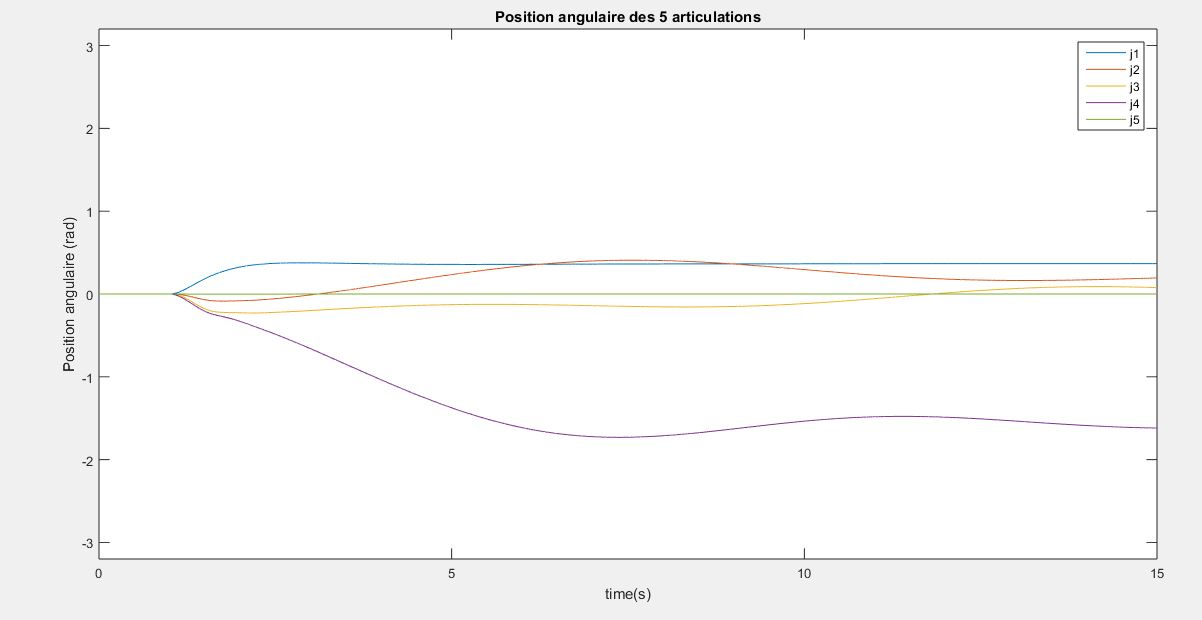
\includegraphics[width=\textwidth]{./PIDtaskartigraph.JPG}
		\caption{Réponse temporelle des positions angulaires à un échelon filtré de consigne pour le système dans l'espace opérationnel.}
		\label{fig:PIDtaskartigraph}
	\end{center}
\end{figure}

\begin{figure}[H]
	\begin{center}	
		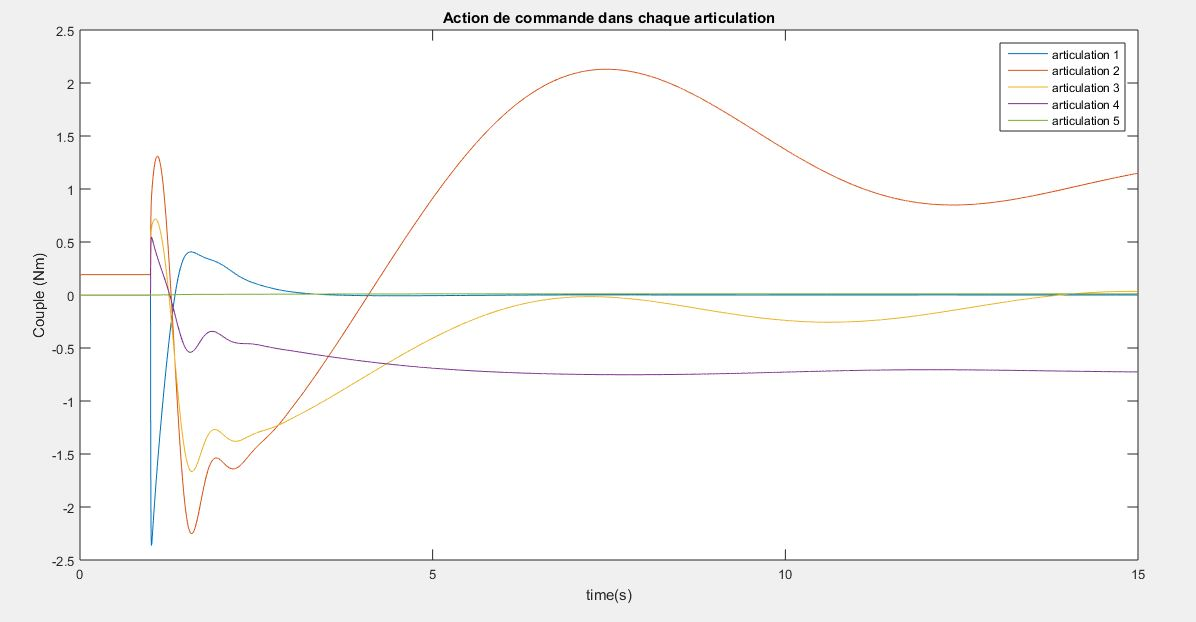
\includegraphics[width=\textwidth]{./PIDtaskcontgraph.JPG}
		\caption{Efforts de contrôle pour le système dans l'espace opérationnel.}
		\label{fig:PIDtaskcontgraph}
	\end{center}
\end{figure}

Dans ce cas, on peut voir que le robot est un peu plus lente pour arriver au point de consigne, et il n'arruve pas exactement au point, il reste une erreur en régime permanent, même avec un tèrme intégrale dans le contrôleur. Pour les positions angulaires les efforts de contrôle, on peut voir qu'ils sont bien limités, mais ils ne stabilisent jamais.

Alors, pour la suite on doit fixer ces problèmes et commencer à générer des consignes pour l'orientation d'outil aussi avant de l'intégrer avec le générateur de trajectoire.